\documentclass[handout]{beamer}

\usepackage{fontspec} 
% \usepackage{lsp-makros}
\useoutertheme{lsp}

\usepackage{lsptitle}

\def\two@digits#1{\ifnum#1<10 0\fi\number#1}
\def\mytoday{\two@digits{\number\day}.\two@digits{\number\month}.\number\year}


\usepackage{xspace,multicol}
\newcommand{\latex}{\LaTeX\xspace}
\usepackage{tikz}


\newcounter{lastpagemainpart}
\footnotesep0pt
\renewcommand{\footnoterule}{}
\usefootnotetemplate{
  \noindent
  \insertfootnotemark\insertfootnotetext}

\let\beamerfn=\footnote
\renewcommand{\footnote}[1]{%
\let\oldfnsize=\footnotesize%
\let\footnotesize=\tiny%
\beamerfn<\thebeamerpauses->{#1}%
\let\footnotesize=\oldfnsize}


\date{26.2.2018 Bergisch-Gladbach}

\usepackage{eurosym}  
 
\renewcommand{\centerline}[1]{\hfill#1\hfill\hfill\mbox{}}


\title{\mbox{Übergang vom Community-Projekt} \mbox{zum tragfähigen Geschäftsmodell}}
% \institute{FU Berlin}
\author[LangSci]{\mbox{Sebastian Nordhoff, Language Science Press, HU Berlin}
% \mbox{\tiny\url{https://github.com/langsci/lsp-presentations/blob/master/oat2017books/presentation.pdf}}
}



\begin{document}
\lspbeamertitle

\frame{
\frametitle{Outline}
\tableofcontents
}
\section{Hintergrund}
\frame{
\frametitle{Sprachwissenschaft}
\begin{itemize}
 \item   Allgemeine Sprachwissenschaft relativ klein, aber mit Ausstrahlungen in Germanistik, Anglistik, Romanistik
 \item   25\,000 Linguisten weltweit
 \item   Bücher und Zeitschriften
 \item Buchpreise 100-200 EUR 
 \item Auflage ca. 200
 \item Druckkostenzuschüsse unüblich
 \item   Peer Review 
 \item   ``Die naturwissenschaftlichste unter den Geisteswissenschaften''
\end{itemize}
}


\frame{
\frametitle{Sebastian Nordhoff}
\begin{columns}
  \begin{column}{2cm}
   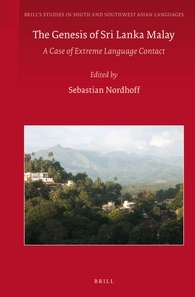
\includegraphics[width=2.5cm]{./pics/brill.jpg}
  \end{column}
  \begin{column}{7.5cm}
    \begin{itemize}
    \item PhD 2009, Universiteit van Amsterdam 
    \item \textit{A grammar of Upcountry Sri Lanka Malay}
    \item 3 Sammelbände, ca. 25 Artikel
    \item Linked Open Data am MPI für Evolutionäre Anthropologie in Leipzig (2009-12)
    \end{itemize}
  \end{column}
\end{columns}
\begin{itemize}
    \item Glottolog.org: Referenzdatenbank mit  320\,559 Literaturangaben zu 23\,495 Sprachen und Dialekten
    \item Seit 2014 Koordinator Language Science Press  
\end{itemize}
} 


% \section{Language Science Press}
\frame{
\frametitle{Language Science Press}
%   \includegraphics[height=.2\textheight]{./path/to/graphicsfile}
  \begin{itemize}
    \item linguistische Monographien und Sammelbände als CC-BY
    \item  aktiv seit 2014 (FU Berlin), seit 2017 HU Berlin
    \item  20 Reihen,  160 Herausgeber weltweit 
    \item 40 Bücher, 330 Interessensbekundungen
    \item  935 \textit{public supporters} + 305 ``anonyme Unterstützer''
    \item Plan ab 2018: 30 Bücher pro Jahr
    \item bis zu >20.000 Downloads pro Buch
    \item Open-Access-Preis der Deutschen Gesellschaft für Sprachwissenschaft
  \end{itemize}
}

\frame{ 
\frametitle{Was wir publizieren:} 
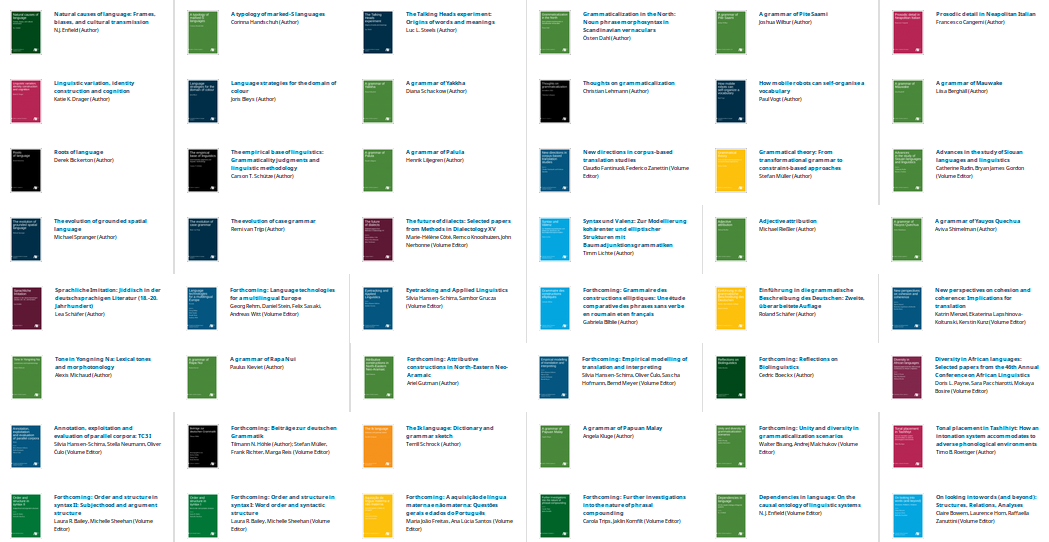
\includegraphics[width=\textwidth]{catalog.png} 
}



\frame{ 
\frametitle{Was wir publizieren:}
\begin{tabular}{ll}
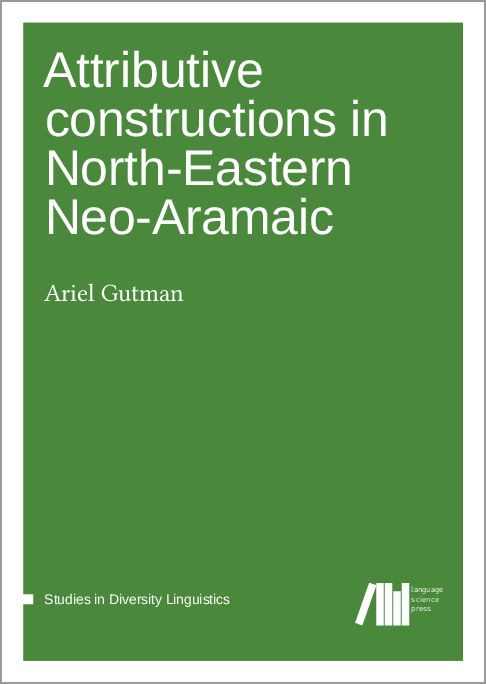
\includegraphics[width=.35\textwidth]{gutman.png}& 
\parbox{.65\textwidth}{
\fbox{
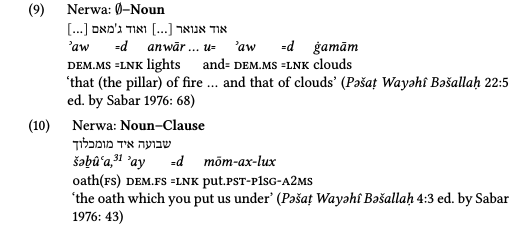
\includegraphics[width=.6\textwidth]{nena.png}  
}
\begin{itemize}
 \item Bücher bis 750 Seiten
 \item teilweise Frucht mehrerer Jahrzehnte Arbeit
 \item Mix zwischen Automatisierung und Maßanfertigung
\end{itemize}

 
\vspace*{6cm}  
}
\end{tabular}
}


% \frame{ 
% \frametitle{Was wir publizieren:}
% \begin{tabular}{ll}
% 
\includegraphics[width=.35\textwidth]{nerbonne.png}& 
% \parbox{.65\textwidth}{
% \fbox{
% 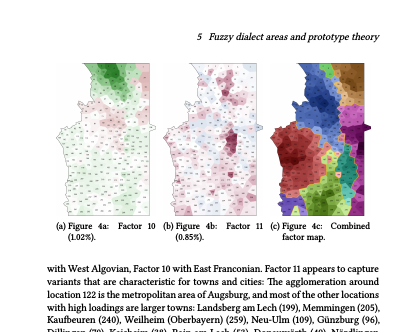
\includegraphics[width=.6\textwidth]{picklmap.png}  
% }
%  
% \vspace*{53mm}  
% }
% \end{tabular}
% }

 


% \frame{ 
% \frametitle{Was wir publizieren:} 
% \begin{tabular}{ll}
% 
\includegraphics[width=.35\textwidth]{mueller.png}& 
% \parbox{.65\textwidth}{
% \fbox{
% 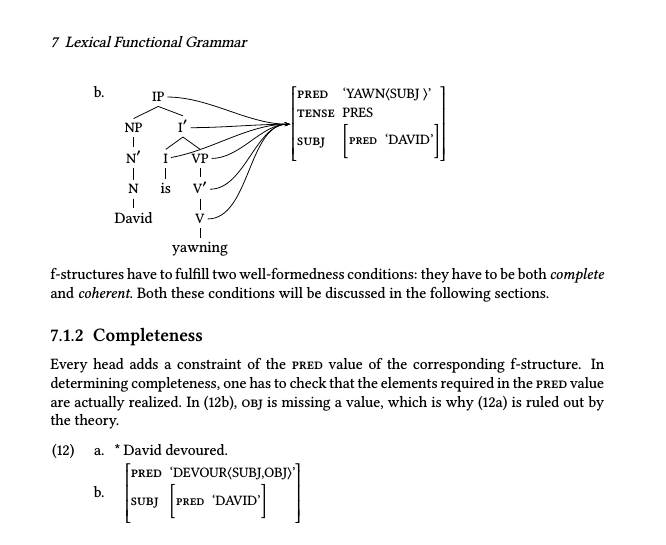
\includegraphics[width=.6\textwidth]{lfg.png}  
% }
%  
% \vspace*{50mm}  
% }
% \end{tabular}
% }

  
\frame{
\frametitle{Timeline}
\begin{itemize}
 \item   2012 erstes Treffen
 \item   2013 DFG-Antrag
 \item   2014-2016 DFG-Projekt
 \item   Seit 2017 an der HU
\end{itemize}
}    
  
\frame{
\frametitle{Prinzipien}
\begin{itemize}
 \item Prinzip der Offenheit
 \item Prinzip der Community 
 \item Prinzip der Schlankheit
\end{itemize}
}  


\section{Prinzipien}
% \subsection{Prinzip der Offenheit}

\frame{
\frametitle{Prinzip der Offenheit}
%   \includegraphics[height=.2\textheight]{./path/to/graphicsfile}
  \begin{itemize}
    \item  Nur FLOSS, nur CC-BY, transparente Kalkulationen
  \end{itemize}
  
  
\includegraphics[width=3cm]{omp.png} 
  
\includegraphics[width=3.5cm]{github.png} 
  
\includegraphics[width=4cm]{paperhive.png}
  
  
\includegraphics[width=3cm]{overleaf.png}
  
\includegraphics[width=3cm]{ctan.png}
  
\includegraphics[width=3cm]{oapen.png}
  
\includegraphics[width=3cm]{doab.png}
}
 

% \subsection{Prinzip der Community}
\frame{
\frametitle{Prinzip der Community}
%   \includegraphics[height=.2\textheight]{./path/to/graphicsfile}
  ~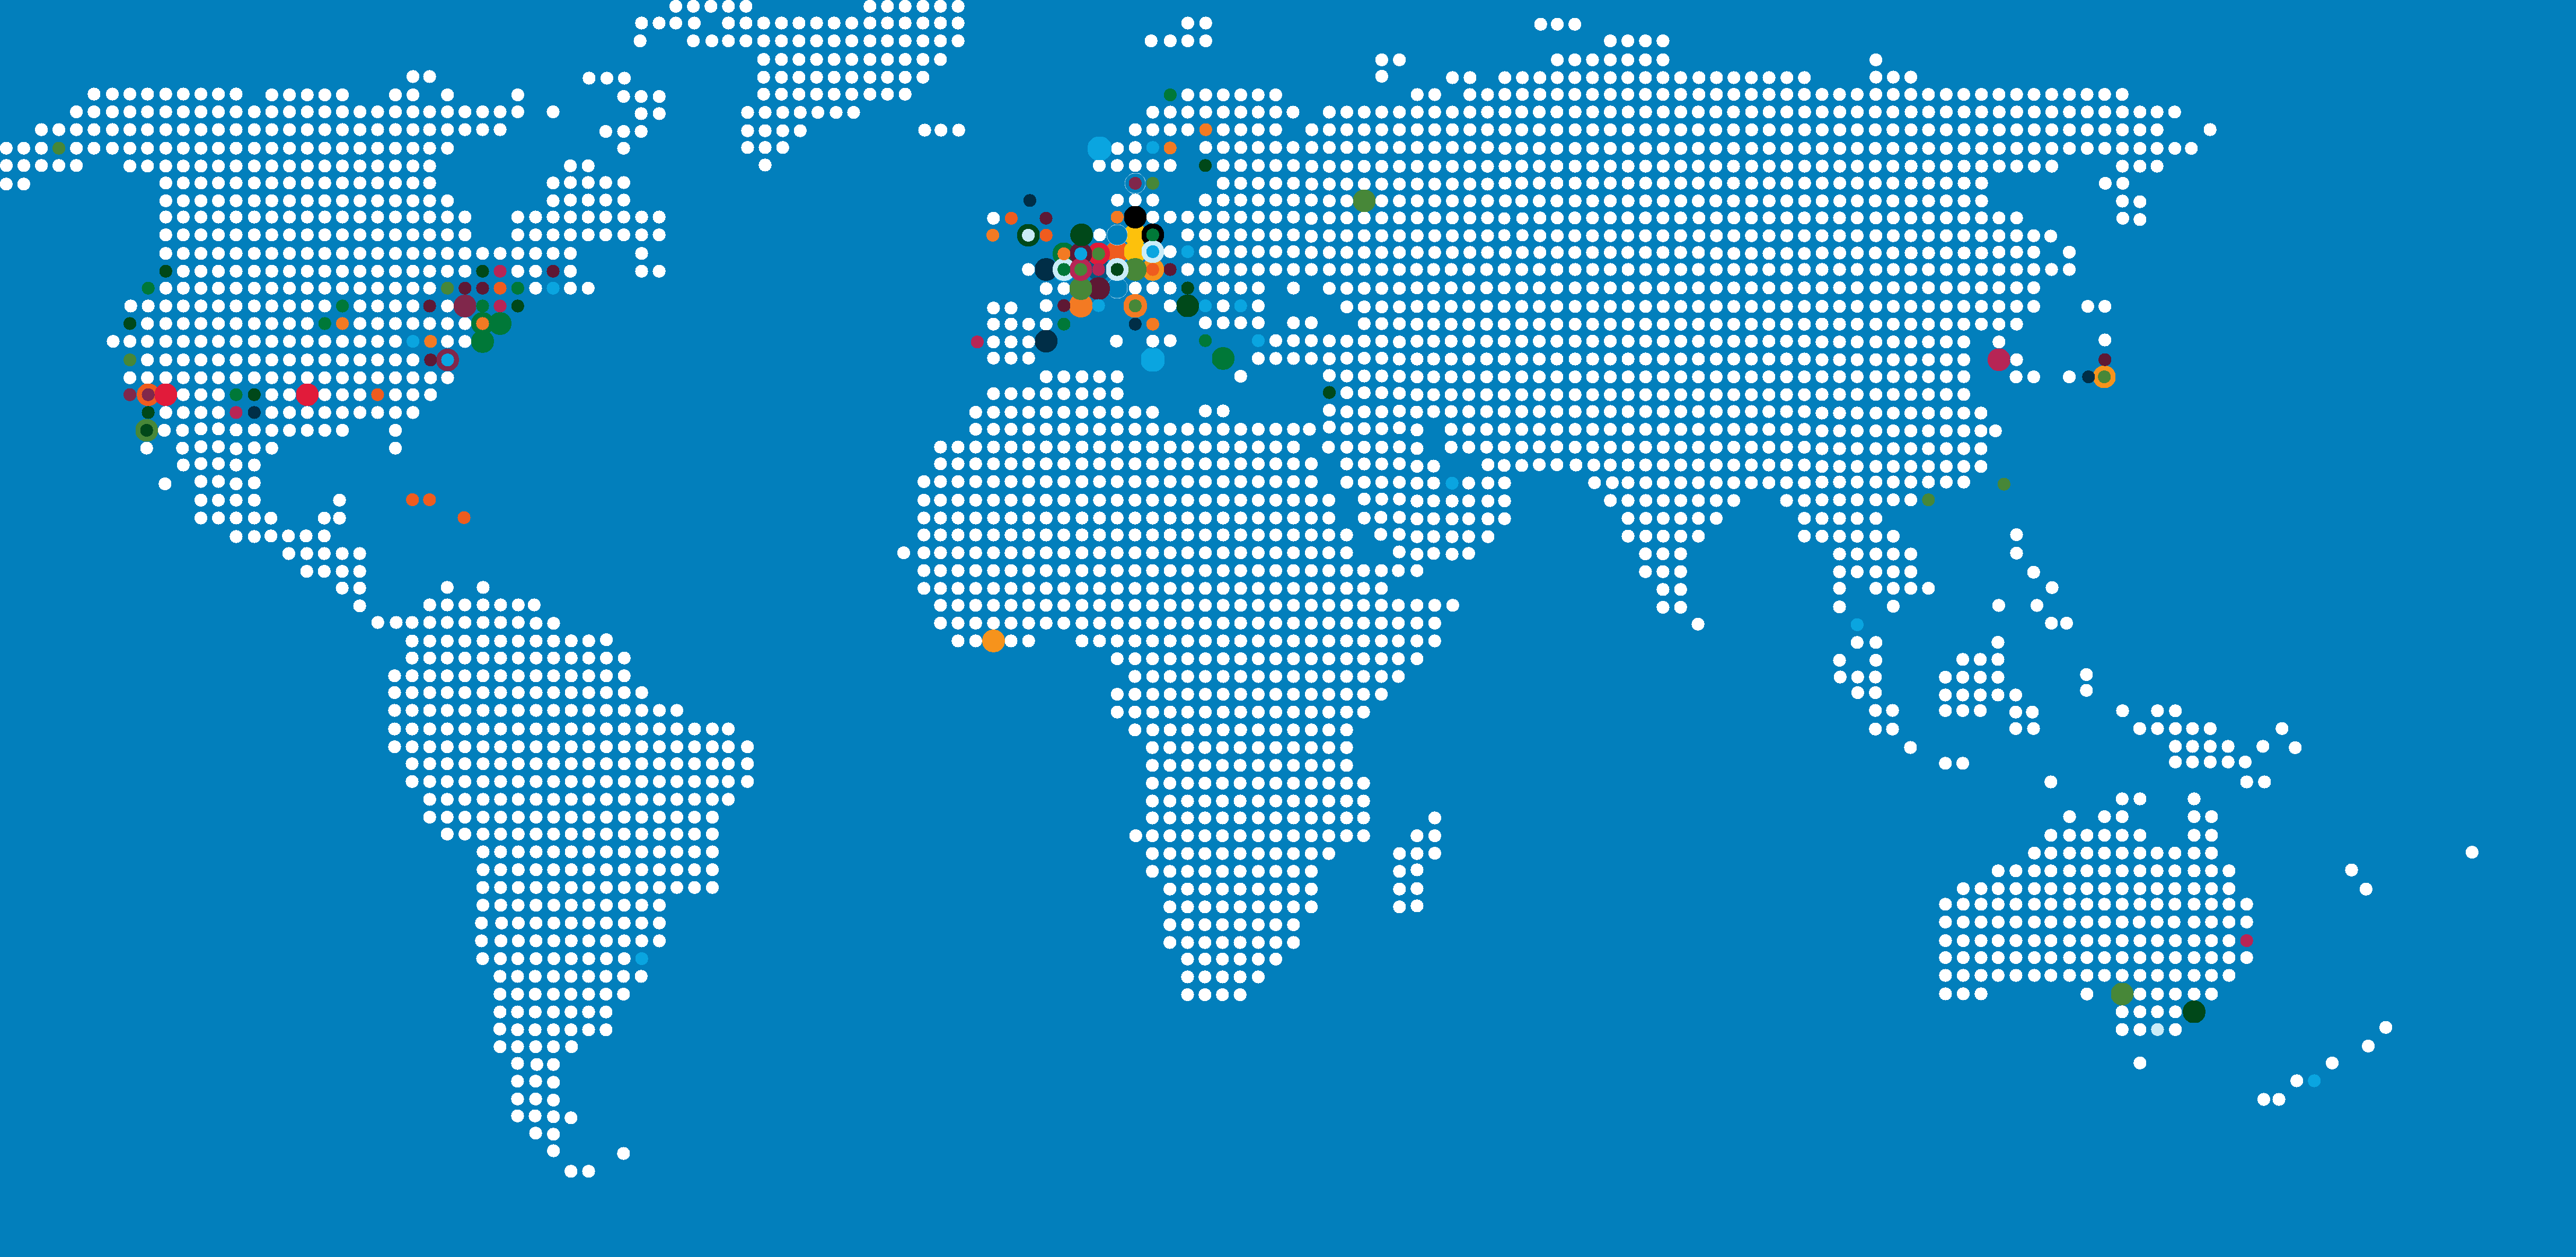
\includegraphics[width=.95\textwidth]{WORLDMAPDOTSdots.png}
  \begin{itemize}
    \item weltweit, autark, dezentral, bottom-up
    \item own the brands (anders als LivingReviews, SSRN,  etc)
    \item share the source
    \begin{itemize}
     \item  Templates, Quelldateien, Geschäftsprozesse, Kalkulationen
    \end{itemize}
  \end{itemize}
}


% \subsection{Prinzip der Schlankheit}    

\frame{
\frametitle{Prinzip der Schlankheit}
%   \includegraphics[height=.2\textheight]{./path/to/graphicsfile}
  \begin{itemize}
    \item keine Legacy-Software
    \item keine Lagerhaltung
    \item kein Vertrieb
    \item keine IT für Paywalls, Registrierung
    \item kein Marketing 
    \item keine Buchstände
    \item keine komplizierten Autorenverträge 
    \item keine Tantiemen\\$\to$ born digital
  \end{itemize}
}

\section{Prestige}
\frame{
\frametitle{Prestige}
\begin{itemize}
\item Motivationsgefüge der Autoren berücksichtigen
\begin{itemize}
 \item Karma $\Longleftrightarrow$ Karrierechancen
\end{itemize}
\item Karrierechancen sind ein wesentlicher Faktor bei der Wahl eines Verlages 
\item Open Access kann nur dann Bestand haben, wenn die Karrierechancen nicht darunter leiden
\item Karrierechancen korrelieren mit Prestige der Veröffentlichungsorte
\item $\to$ ein neuer Verlag muss sehr schnell sehr viel Prestige aufbauen
\end{itemize}
}

\frame{
\frametitle{Quellen von Prestige}
\begin{enumerate}
 \item Prominente Unterstützer
 \item Menge an Unterstützern
 \item Qualität der Bücher
 \item Selektivität/Exklusivität
\end{enumerate}
}

\frame{
\frametitle{Prominente Unterstützer}

    \parbox{.4\textwidth}{
      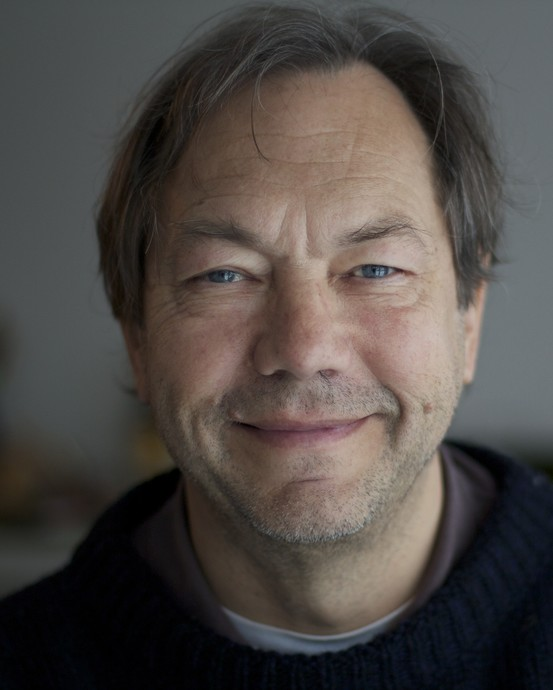
\includegraphics[height=.8\textheight]{pics/steels-s.jpg}
      
      Luc Steels
      }
    \parbox{.4\textwidth}{
      ~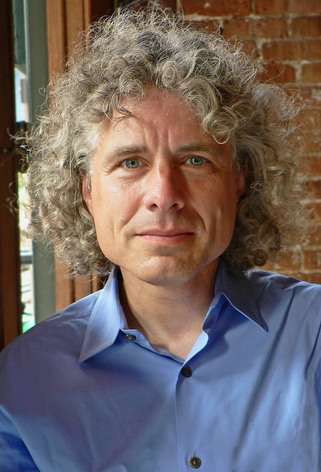
\includegraphics[height=.8\textheight]{pics/pinker-s.jpg}
      
      Steven Pinker
    }
}



\frame{
\frametitle{Menge an Unterstützern}
\begin{itemize}
\item    öffentlich einsehbare Supporterseite 
\begin{itemize}
 \item \url{http://langsci-press.org/supporters}
\end{itemize}
\item    Mailingliste
\item    ``Pledge to Publish'' vor Projektstart
\item    kritische Masse war schon vor Projektstart erreicht
\item    Start auf der Jahrestagung der Deutschen Gesellschaft für Sprachwissenschaft 
mit dem ersten Buch 7 Tage nach Projektbeginn
\end{itemize}
}


\frame{
\frametitle{Formale Qualität}
\begin{itemize}
\item Einheitliches reihenübergreifendes Erscheinungsbild 
\item \LaTeX
\item Ligaturen 
\parbox{.3\textwidth}{
\includegraphics[width=.3\textwidth]{pics/affin.png}}
 \item recht strenges Stylesheet
\end{itemize}
}

\frame{
\frametitle{Formale Qualität}
\begin{itemize}
\item Chinesisch, Hebräisch, Arabisch
\item diverse fachspezifische Erweiterungen
\item Namensindex, Sprachindex, thematischer Index
\item klickbare Querverweise
\item Print-on-Demand
\begin{itemize}
  \item ISBNs
  \item DOIs, auch auf Kapitelebene
 \item theoretisch noch Prestige durch hohen Preis im dreistelligen Bereich
 \item bei Language Science Press ca. 30 EUR/Buch
\end{itemize}

\end{itemize}
}

\frame{
\frametitle{Inhaltliche Qualität}
\begin{itemize}
\item traditioneller Peer Review
\begin{itemize}
 \item organisiert vom Reihenherausgeber zusammen mit Editorial Board
\end{itemize}
\item keine Dissertationen (Selektivität)
\item proaktive Kommunikation von Annahme-/Ablehnungraten
\end{itemize}
}

\frame{
\frametitle{Innovation}
\begin{itemize}
 \item GitHub 
 \item Overleaf 
 \item PaperHive
\end{itemize}
}
\section{Finanzierung}

\frame{
\frametitle{Finanzierung}
\begin{itemize}
 \item DFG-Projekt mit 50\%-Stelle für Betriebswirtin 
 \item Vision, Mission, Stakeholder-Analyse, Wertversprechen, Einnahmearten, Kostendeckungsbeiträge
 \item Overhead pro Kostenart
 \item Benötigt: ca. 100\,000 EUR p/a
 \item Finanzierungsmöglichkeiten \pause
 \begin{itemize}

 \item Consortia\pause
 \item Printmarge \pause 
 \item Autorengebühren\pause 
 \item Spenden\pause
 \item Mitgliedschaften  
 \end{itemize}
\end{itemize}
}

\frame{
\frametitle{Knowledge Unlatched}
\begin{itemize}
 \item Verteilte Finanzierung: 100 Bibliotheken weltweit zu 1000 EUR/Jahr 
 \item Leistung: 30 Bücher/Jahr, peer-reviewed, CC-BY
 \item 3-jährige Perioden
 \item je nach Bibliothek sehr schnell oder sehr langwierig
\end{itemize}

\includegraphics[width=10cm]{pics/funding.png}
}
\section{Übertragbarkeit}

% \frame{
% \frametitle{Voraussetzungen} 
%   \begin{itemize}
%   \item Community-Building
%   \item keine Gewinnerzielungsabsicht
%   \item kein Anspruch auf Verwertungsrechtemonopol
%   \item verteilte Finanzierung (konkret: Knowledge Unlatched)
%   \item klares inhaltliches Profil
%   \item Buchmenge überschaubar und vorhersagbar 
%   \item Anerkennungskultur      
%   \end{itemize} 
% }

\frame{
\frametitle{Language Science Press zum Nachkochen}
\begin{itemize}
 \item OpenAire-Projekt: \textit{Full disclosure: replicable strategies for book publications supplemented with empirical data}
 \begin{itemize}
 \item Geschäftsmodell zum Nachlesen als CC-BY 
 \item HowTo zum Nachbauen als CC-BY
 \item Geschäftszahlen (Downloads, Verkäufe) als CC-0
 \item Spreadsheet zum Nachrechnen
 \item Verfügbar 2018/06
 \end{itemize}
\end{itemize}

\includegraphics[width=2cm]{pics/openaire.png}
}

\section{Diskussion}

\frame{
\frametitle{Diskussion}
\begin{itemize}
  \item OA-``Heilsversprechen''
 \begin{itemize}
 \item Haben durch OA mehr Menschen Zugang? 
 \item Ist OA billiger? 
 \item Ist OA demokratischer? 
 \end{itemize}
 \item Was sind die Voraussetzungen innerhalb eines Fachbereichs für eine erfolgreiche OA-Transformation? 
 \begin{itemize}
  \item Hochenergiephysik (SCOAP3)
  \item Sprachwissenschaft (LingOA, Glossa, Language Science Press)
  \item ???
 \end{itemize}
 \item Sammlungsauftrag von Bibliotheken vs. dezentrale Finanzierung von Publikationsplattformen
\end{itemize}
}

\end{document}
